\documentclass[10pt]{article}
\usepackage{fullpage, graphicx, url}
\usepackage[colorlinks=true]{hyperref}
\setlength{\parskip}{1ex}
\setlength{\parindent}{0ex}
\begin{document}
\title{Brick 1.2 Test Suite}
\author{}
\date{}
\maketitle

\section*{Oscillators}

Not all oscillators are made equal. Here we see that the built-in
          trigonometric functions in the C++ standard library CMath build up harmonics
          and noise when the values of the input grow to high.
        

\subsection*{Input Files}

\begin{verbatim}
_Sweep80s_Precise.aiff
_Sweep80s_Machine.aiff
_Sweep80s_CMath.aiff
_Tone80s_Recursive.aiff
\end{verbatim}

\subsection*{Notes}

The recurrence relation used for the tone in Figure 4 is of the form:

\begin{verbatim}
sin[n * f] = a[n] = 2 cos(f) a[n - 1] - a[n - 2]
a[-1] = sin(-f)
a[-2] = sin(-2f)
\end{verbatim}

The formula is exceptionally stable over long iterations and
          appears to neither drift in frequency nor accumulate noise. In this case, f is
          the two-pi times divided by the Euler constant, 2 Pi \slash  e. This frequency was picked since it is irrational and therefore will not exactly repeat.

\begin{figure} \begin{center} \setlength\fboxrule{0.01in}\fbox{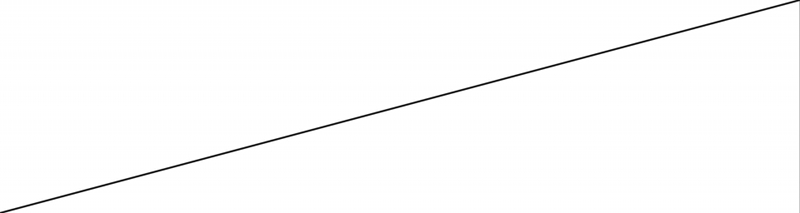
\includegraphics[width=5.5in]{_Sweep80s_Precise_.png}}\end{center} \caption{80-second sweep implemented using arbitrary precision in Mathematica.} \end{figure}


\begin{figure} \begin{center} \setlength\fboxrule{0.01in}\fbox{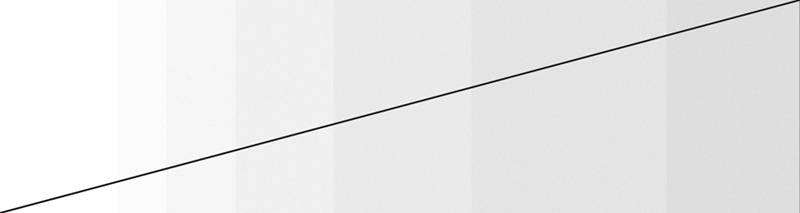
\includegraphics[width=5.5in]{_Sweep80s_Machine_.png}}\end{center} \caption{80-second sweep implemented using MachinePrecision in Mathematica.} \end{figure}


\begin{figure} \begin{center} \setlength\fboxrule{0.01in}\fbox{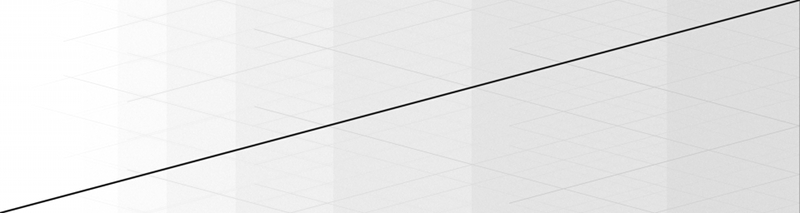
\includegraphics[width=5.5in]{_Sweep80s_CMath_.png}}\end{center} \caption{80-second sweep implemented using the sin() function from the cmath library.} \end{figure}


\begin{figure} \begin{center} \setlength\fboxrule{0.01in}\fbox{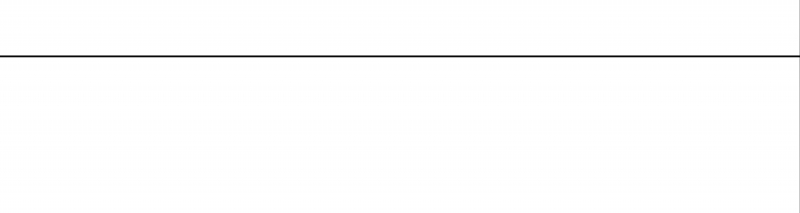
\includegraphics[width=5.5in]{_Tone80s_Recursive_.png}}\end{center} \caption{80-second tone implemented using the sine recurrence relation.} \end{figure}

\end{document}